%---------------------------------------------------------------------------%
%-                                                                         -%
%-                          Beamer Template                                -%
%-                                                                         -%
%---------------------------------------------------------------------------%
%- Copyright (C) Huangrui Mo <huangrui.mo@gmail.com> 
%- This is free software: you can redistribute it and/or modify it
%- under the terms of the GNU General Public License as published by
%- the Free Software Foundation, either version 3 of the License, or
%- (at your option) any later version.
%---------------------------------------------------------------------------%
%->> Document class declaration
%---------------------------------------------------------------------------%
\documentclass[compress,table,aspectratio=169,xcolor={usenames,dvipsnames}]{beamer}%
%- Multiple options:
%- [<t|c|b>]% vertical alignment for content, vertically centered is default
%- [<slidestop|slidescentered>]% set frame titles position
%- [compress]% reduce the navigate bars
%- [<red|blue|brown|blackandwhite>]% set navigate bar color
%- [<10pt|11pt|12pt|14pt|17pt>]% set font size for normal text, 11pt is default
%- [table]% support tables
%- [aspectratio=169]% set aspect ratio to 16:9, and frame size to 160mm by 90mm
%- [aspectratio=1610]% set aspect ratio to 16:10, and frame size to 160mm by 100mm
%- [aspectratio=MN]% set aspect ratio to M:N, and frame size to 10*M mm by 10*N mm
%- [xcolor={usenames,dvipsnames}]% issue options to xcolor via a beamer-option
%- Manually adjust aspect ratio: design to 4x3, then expand to target, and live with empty space
%- \documentclass[aspectratio=169]{beamer}
%-     \beamertemplatenavigationsymbolsempty%
%-     \usepackage{pdfpages}%
%- \begin{document}
%-     \setbeamercolor{background canvas}{bg=}%
%-     \includepdf[pages=-]{my-original-presentation.pdf}%
%- \end{document}
%- The default font size may seem small, but the actual size of each frame size is
%- by default just 128mm by 96mm and the viewer application enlarges the frame and font.
%- By specifying a default font size smaller than 11pt one can put more onto each slide,
%- by specifying a larger font size one can fit on less.
%---------------------------------------------------------------------------%
%->> Document settings
%---------------------------------------------------------------------------%
\usepackage[biber,authoryear,tikz,table,xlink]{Style/artrabeamer}% document settings
%- usage: \usepackage[option1,option2,...,optionN]{artrabeamer}
%- Multiple optional arguments:
%- [CJK]% Chinese environment support
%- [bibtex|biber]% set bibliography processor and package
%- [<numbered|authoryear|alpha>]% set citation and reference style
%- <numbered>: textual: Jones [1]; parenthetical: [1]
%- <authoryear>: textual: Jones (1995); parenthetical: (Jones, 1995)
%- <alpha>: textual: not available; parenthetical: [Jon95]
%- [tikz]% provide complex diagrams via tikz package
%- [table]% provide complex tables via ctable package
%- [list]% provide enhanced list environments for algorithm and coding
%- [math]% enable some extra math packages
%- [showonlynote]% show note pages only
%- [showsecnote]% show note pages on second screen
%- [handout]% enable handout output
%- [xlink]% disable link colors
\usepackage{Style/artracom}% user defined commands
\usepackage{graphicx}
\usepackage{amsmath}
\usepackage{longtable}
\usepackage{gensymb}
\usepackage{enumerate}
\usepackage{varwidth}
\usepackage{float}
\usepackage{nonfloat}
\usepackage{soul}
\usepackage{ulem}
% \usepackage{multicol}
% \usepackage{afterpage}

\newcommand\Ra{\mathrm{Ra}}
\newcommand\Pran{\mathrm{Pr}}
\newcommand\Rac{\mathrm{Ra}_{\mathrm{c}}}
\newcommand\Ek{\mathrm{Ek}}
\newcommand\Ro{\mathrm{Ro}}
\newcommand\Nu{\mathrm{Nu}}
\newcommand\Sc{\mathrm{Sc}}

\newcommand\eps{\varepsilon}
\renewcommand\L {\mathcal{L}}

\newcommand{\n}{\\ \nonumber \\ }
\newcommand{\nn}{\nonumber}
\newcommand{\nnn}{\\ \nonumber \\ \nonumber}

\newcommand\ie{\textit{i.e.},~}
\newcommand\eg{\textit{e.g.},~}
\newcommand{\omicron}{o}

\newcommand{\pd}[1]{\partial_{#1}}
\renewcommand{\vec}[1]{\boldsymbol{#1}}
\newcommand{\M}[1]{\mathbf{#1}}
\newcommand{\grad}{\vec{\nabla}}
\newcommand{\cross}{\vec{\times}}
\newcommand{\laplacian}{\nabla^2}

\newcommand{\sump}[2]{\sideset{}{'}\sum_{{#1}=0}^{#2}}

\newcommand{\eq}[1]{(\ref{#1})}
\newcommand{\eqs}[2]{(\ref{#1})~\&~(\ref{#2})}
\newcommand{\eqss}[2]{(\ref{#1})--(\ref{#2})}

\newcommand{\Eq}[1]{Eq.~(\ref{#1})}
\newcommand{\Eqs}[2]{Eqs.~(\ref{#1})~\&~(\ref{#2})}
\newcommand{\Eqss}[2]{Eqs.~(\ref{#1})--(\ref{#2})}

\newcommand{\fig}[1]{Fig.~(\ref{#1})}
\newcommand{\figs}[2]{Figs.~(\ref{#1})~\&~(\ref{#2})}
\newcommand{\T}{{\cal T}}
\newcommand{\Z}{{\cal Z}}

%---------------------------------------------------------------------------%
%->> Document inclusion
%---------------------------------------------------------------------------%
%\includeonly{Tex/Sec_Introduction}% selected files compilation
%\includeonlylecture{lecture label}% selected lectures compilation
%---------------------------------------------------------------------------%
%->> Theme settings
%---------------------------------------------------------------------------%
%-
%-> Recommended theme combinations
%-
%- set: [<usetheme>, <useoutertheme>, <useinnertheme>, <usecolortheme>]
%- light: [<CambridgeUS>, <miniframes>, <circle>, <dove|seahorse|beaver|seagull>]
%- light: [<Boadilla|Madrid>, <default>, <circle>, <dove|seahorse|beaver|seagull>]
%- dark: [<Boadilla|Madrid>, <default>, <circle>, <fly|albatross>]
%-
%-> Global themes
%-
\usetheme{CambridgeUS}%
%- Options:
%- [<Boadilla|CambridgeUS|default|...>]
%- It is the complete theme in the sense that they control just about every aspect
%- of a slide's appearance. Think of it as major theme.
%- Theme Matrix (https://www.hartwork.org/beamer-theme-matrix/) contains the
%- various theme and color combinations included with beamer.
%-
%-> Outer themes
%-
%\useoutertheme{}%
%- Options:
%- [<default|infolines|miniframes|smoothbars|sidebar|split|shadow|tree|smoothtree>]
%- An outer theme dictates (roughly) the overall layout of frames. It specifies where
%- any navigational elements should go (like a mini table of contents or navigational
%- mini frames) and what they should look like. Typically, an outer theme specifies
%- how the following elements are rendered:
%- - The headline and footline.
%- - The sidebars.
%- - The logo.
%- - The frame title.
%- The Beamer User Guide explains each theme with examples.
%-
%- *** Miniframes
\useoutertheme[%
    %footline=empty,% suppressed the footline (default).
    %footline=authorinstitute,% shows the author's name and the institute in the footline.
    %footline=authortitle,% shows the author's name and the title in the footline.
    %footline=institutetitle,% shows the institute and the title in the footline.
    %footline=authorinstitutetitle,% shows all three in the footline.
    subsection=false,% shows or suppresses line showing the subsection in the headline.
]{miniframes}%
%-
%- *** Sidebar
%\useoutertheme[%
%    %left,% sidebar links.
%    %right,% sidebar rechts.
%    %hideallsubsections,% suppresses all subsections.
%    %hideothersubsections,% suppresses all subsections except the current one.
%]{sidebar}%
%-
%-> Inner themes
%-
\useinnertheme{circles}%
%- Options:
%- [<default|circles|rectangles|rounded|inmargin>]
%- An inner theme installs templates that dictate how the following elements are typeset:
%- - Title and part pages.
%- - Itemize environments.
%- - Enumerate environments.
%- - Description environments.
%- - Block environments.
%- - Theorem and proof environments.
%- - Figures and tables.
%- - Footnotes.
%- - Bibliography entries.
%-
%-> Color themes
%-
\usecolortheme{dove}%
%- Options:
%- [<dove|seahorse|beaver|seagull|fly|albatross|...>]
%- Control the colors of title, frame title, itemization bullets,
%- and many other elements of a slide show.
%- More detailed configure:\setbeamercolor{beamer_element}{color} for
%- of Beamer elements, e.g.color setup
%\setbeamercolor{title}{fg=red!80!black,bg=red!20!white}
%\setbeamercolor{frametitle}{fg=blue,bg=yellow}
%---------------------------------------------------------------------------%
%->> Configuration
%---------------------------------------------------------------------------%
%-
%-> Set templates
%-
%- As a user of the beamer class you typically do not 'use' or 'invoke'
%- templates yourself, directly. For example, the frame title template
%- is automatically invoked by beamer somewhere deep inside the frame
%- typesetting process. The same is true of most other templates.
%- However, if, for whatever reason, you wish to invoke a template
%- yourself, you can use the following command.
%-\setbeamertemplate{some beamer element}{your definition for this template}
%-
%- *** Headline and footline
%\setbeamertemplate{headline}[infolines theme]
%\setbeamertemplate{footline}[page number]
%- Options: {},[default],[infolines theme],[miniframes theme],[frame number],
%-          [page number],[text line]{ text },...
%- Example for redefine the footline:
%-
%- First define some "beamer color" entries:
%\setbeamercolor{myentry1}{fg=black,bg=red!20}
%\setbeamercolor{myentry2}{fg=black,bg=red!30}
%\setbeamercolor{myentry3}{fg=black,bg=red!40}
%- Syntax for \begin{beamercolorbox}[options]{beamer color} ... \end{beamercolorbox}.
%- footline:
%\setbeamertemplate{footline}{
%  \leavevmode%
%  \hbox{%
%  \begin{beamercolorbox}[wd=.333333\paperwidth,ht=2.25ex,dp=1ex,center]{myentry1}%
%-    \usebeamerfont{author in head/foot}\insertshortauthor
%  \end{beamercolorbox}%
%  \begin{beamercolorbox}[wd=.333333\paperwidth,ht=2.25ex,dp=1ex,center]{myentry2}%
%-    \usebeamerfont{title in head/foot}\insertshorttitle
%  \end{beamercolorbox}%
%  \begin{beamercolorbox}[wd=.333333\paperwidth,ht=2.25ex,dp=1ex,right]{myentry3}%
%-    \usebeamerfont{date in head/foot}\insertshortdate{}\hspace*{2em}
%    \insertframenumber{} / \inserttotalframenumber\hspace*{2ex}
%  \end{beamercolorbox}}%
%  \vskip0pt%
%}
%- headline:
%\setbeamertemplate{headline}{
%  \leavevmode%
%  \hbox{%
%  \begin{beamercolorbox}[wd=.5\paperwidth,ht=2.65ex,dp=1.5ex,right]{myentry1}%
%    \usebeamerfont{section in head/foot}\insertsectionhead\hspace*{2ex}
%  \end{beamercolorbox}%
%  \begin{beamercolorbox}[wd=.5\paperwidth,ht=2.65ex,dp=1.5ex,left]{myentry3}%
%    \usebeamerfont{subsection in head/foot}\hspace*{2ex}\insertsubsectionhead
%  \end{beamercolorbox}}%
%  \vskip0pt%
%}
%- Change the footer/footline of a single frame in Beamer: use {} to confine effect domain.
%- The \leavevmode ensures that the vertical mode is ended and horizontal mode is entered. 
%- In vertical mode, TeX stacks horizontal boxes vertically, whereas in horizontal mode, 
%- they are taken as part of the text line. Use \leavevmode for all macros which could be 
%- used at the begin of the paragraph and add horizontal boxes by themselves.
%-
%- *** Outline setting
%\AtBeginPart% [<Lecture|Part|Section>]% insert content at the beginning of each element
%{%
%    \frame[plain]{\partpage}% [<partpage|sectionpage>][<\insertlecture|\insertpart|\insertsection>]
%    \begin{frame}[plain]%
%        \frametitle{Outline}%
%        {%
%            \tableofcontents[sectionstyle=show/shaded,subsectionstyle=show/show/shaded]%
%        }%
%    \end{frame}%
%}
%- - sectionstyle=<style for current section>/<style for other sections>
%- - subsectionstyle=<style for current subsection>/<style for other
%-   subsections in current section>/<style for subsections in other sections>
%- - Allowed <styles> are show, shaded, and hide.
%- Other options:
%- - currentsection, equal to: sectionstyle=show/shaded,subsectionstyle=show/show/shaded
%- - currentsubsection, equal to: subsectionstyle=show/shaded.
%- - firstsection=<section number> specifies which section should be numbered as section "1."
%-   This is useful if you have a first section (like an overview section) that should not
%-   receive a number.
%- - hideallsubsections, equal to: subsectionstyle=hide.
%- - pausesections, causes a \pause command to be issued before each section.
%-   This is useful if you wish to show the table of contents in an incremental way.
%-
%- *** Navigation symbols
\setbeamertemplate{navigation symbols}{}% suppresses all navigation symbols.
%\setbeamertemplate{navigation symbols}[only frame symbol]% only for navigating frames.
%-
%- *** Frame title
%\setbeamertemplate{frametitle}[default][left]% left, center, right
%-
%- *** Background
%\setbeamertemplate{background}[grid][step=\grid,color=blue]
%\setbeamertemplate{background canvas}[default]
%\setbeamertemplate{background canvas}[vertical shading][bottom=red!20,top=yellow!30]
%\setbeamertemplate{background canvas}{\includegraphics[width=\paperwidth,height=\paperheight]{alps.jpg}}
%\tikzart[t=c]{cover_front_thu_cce}
%\tikzart[t=c]{cover_composite_tonemapped}[trim=0mm 100mm 0mm 0mm,clip]
%- The aspect ratio of a Beamer slide is 4:3 therefore it's best
%- if your background image has the same aspect ratio. Otherwise
%- your image will be distorted when it's stretched to cover the
%- slide from edge to edge.
%- To limit the background setting to a single slide, enclose the
% \setbeamertemplate{background canvas}{...} command in braces,
%- as in:
%-
%{% brace to limit the scope of \setbeamertemplate
%\setbeamertemplate{navigation symbols}{}% optionally hide navigation buttons
%\setbeamertemplate{background canvas}{\includegraphics
%	[width=\paperwidth,height=\paperheight]{alps.jpg}}
%\begin{frame}[plain]
%...
%\end{frame}
%}% closing brace
%-
%- *** Margin sizes
%\setbeamersize{text margin left=2em,text margin right=2em}
%-
%- *** Itemizations, enumerations, and descriptions
%\setbeamertemplate{itemize items}[triangle]
%- Options: [<circle|triangle|square|ball>].
%\setbeamertemplate{enumerate items}[default]
%- Options:
%- [default]% numbered
%- [sections numbered]% section numbered, subsections are not numbered.
%- [subsections numbered]% subsections are numbered, but not the sections.
%- [circle]% numbered circles before section, not subsection.
%- [square]% numbered squares before section. unnumbered squares before subsections.
%- [ball]% similar to square, but use balls.
%- [ball unnumbered]% similar to ball, except that no numbering is used.
%-
%- *** Block environments
%\setbeamertemplate{blocks}[rounded][shadow=true]
%- Types:
%- "theorem", "corollary", "definition" in structure color frame.
%- "examples" in green color frame.
%- "block" in structure color frame with your own title.
%- "alertblock" in alert color frame with your own title.
%-
%- *** Theorem environments
%\setbeamertemplate{theorems}[normal font]
%- Options: [<default|normal font|numbered|ams style>].
%-
%- *** Figures and tables
%\setbeamertemplate{caption}[default]
%- Options:
%- [default]% typesets the caption name (a word like 'Figure' or 'Abbildung' or 'Table')
%- [numbered]% adds the figure or table number to the caption.
%- [caption name own line].
%-
%- *** Adding sections and subsections
%\setbeamertemplate{sections/subsections in toc}[square]
%- Options: [<default|sections numbered|subsections numbered>]
%-          [<circle|square|ball|ball unnumbered>]
%-
%- *** Bibliography
\setbeamertemplate{bibliography item}{}% remove the icon
%-
%-> Fonts
%-
%- Set fonts used for different elements of a slide via Beamer's Font Management.
%- Rules:
%\setbeamerfont{some beamer element}{size=\large}
%- Add * to the command to first completely "reset" the font attributes.
%- Options:
%- parent=structure,size=\large,series=\bfseries,shape=\itshape,family=\sffamily.
%- Explains: there are three familis of font
%- family: \rmfamily(serif) or \sffamily(sans serif), or \ttfamily(monospace).
%- Each family has its own font characteristics, i.e., font properties.
%- shapes: \itshape, \slshape, \scshape, or \upshape.
%- series(light, bold,...): \bfseries, \mdseries.
%-
%- *** Structure font
%\setbeamerfont{structure}{}
%\setbeamerfont{tiny structure}{size=\tiny}
%-
%- *** Normal font
%\setbeamerfont{normal text}{parent=structure,size=\small}% ignored currently
%\setbeamerfont{alerted text}{}
%\setbeamerfont{example text}{}
%-
%- *** Projected text font
%\setbeamerfont{projected text}{parent={tiny structure}}
%-
%- *** Titlepage font
%\setbeamerfont{title}{parent=structure, size=\large}% shape=\itshape,family=\rmfamily
%\setbeamerfont{title in head/foot}{parent=title, size=\tiny}
%\setbeamerfont{subtitle}{parent=title, size=\normalsize}
%\setbeamerfont{author}{parent=title, size=\normalsize}
%\setbeamerfont{author in head/foot}{parent=title, size=\tiny}
\setbeamerfont{institute}{parent=structure, size=\normalsize, series=\mdseries}
%\setbeamerfont{institute in head/foot}{parent=title, size=\tiny}
%\setbeamerfont{date}{parent=institute}
%\setbeamerfont{date in head/foot}{parent=title, size=\tiny}
%-
%- *** Frame title font
\setbeamerfont{frametitle}{parent=structure,size=\large}
%\setbeamerfont{framesubtitle}{parent=frametitle,size=\footnotesize}
%-
%- *** Part fonts
%\setbeamerfont{part name}{size=\Large}
%\setbeamerfont{part title}{parent=title}
%-
%- *** Headline and footline font
%\setbeamerfont{headline}{parent={tiny structure}}
%\setbeamerfont{footline}{parent={tiny structure}}
%-
%- *** Caption font
%\setbeamerfont{caption}{size=\small}
%\setbeamerfont{caption name}{size=\small}
%-
%- *** Button font
%\setbeamerfont{button}{size=\tiny}
%-
%-> Transparent effect
%-
%\setbeamercovered{invisible}
%- Options:
%- [invisible]% is the default and causes covered text to disappear.
%- [transparent]% creates shaded instead of hidden overlays.
%- [dynamic]% makes all covered text quite transparent, but in a dynamic way.
%- [highly dynamic]% has the same effect as dynamic, but the effect is stronger.
%\beamerdefaultoverlayspecification{<+->}% uncover everything in a step-wise fashion
%---------------------------------------------------------------------------%
%->> Document content
%---------------------------------------------------------------------------%
%-
%-> Titlepage information
%-
%---------------------------------------------------------------------------%
%->> Document inclusion
%---------------------------------------------------------------------------%
%\includeonly{Tex/Sec_Introduction,Tex/Sec_Method,Tex/Sec_Result,Tex/Sec_Conclusion}% selected files compilation
%\includeonlylecture{lec_present_intro,lec_present_method,lec_present_result,lec_present_conclude}% selected lectures compilation
%\includeonlyframes{fra_current}% selected frames compilation
%---------------------------------------------------------------------------%
%->> Titlepage information
%---------------------------------------------------------------------------%
\title[]% optional, abbreviated title
{\enorcn{Marginally stable thermal equilibria of Rayleigh-B\'enard convection
}{Beamer 报告}}


\author[]% optional, abbreviated authors
{\enorcn{Liam O'Connor}{\large莫晃锐}}

% \institute[]% optional, abbreviated name
% {
%   %\inst{*}%
%   %\enorcn{Mechanical and Mechatronics Engineering, University of Waterloo}{\small 加拿大滑铁卢大学}
%   %\and
%   %\inst{\dag}%
%   %\enorcn{Center for Combustion Energy, Tsinghua University}{\small 清华大学燃烧能源中心}
%   %\and
%   %\inst{+}%
%   \enorcn{Institute of Mechanics, CAS}{中国科学院力学研究所}
% }

\date[]{\enorcn{November 23, 2021}{2021年10月28日}}% or simply: \date{\today}
%\date[IDS 2018]{International Detonation Symposium, 2018}% conference name

\subject{\enorcn{Report by Huangrui Mo}{莫晃锐报告}}% inserted into the PDF information catalog

%\logo{\tikzart[t=p,x=8,y=-6,w=4]{logo_uw}}% on each slide 
\titlegraphic{\tikzart[t=p,x=0,y=-4,w=4]{northwestern-university-logo-vector}}% only on title page
% can also use any field given by \author, \title, \date, \institute, or \tikz to place image in the title page
%\addtobeamertemplate{headline}{}{% on each slide with headline
%    \tikzart[t=p,x=8,y=7,w=4]{logo_uw}
%}
%---------------------------------------------------------------------------%
%
\begin{document}
%-
%-> Frontmatter
%-
%---------------------------------------------------------------------------%
%->> Frontmatter
%---------------------------------------------------------------------------%
%---------------------------------------------------------------------------%
%->> Create titlepage
%---------------------------------------------------------------------------%
%- create the title page, \frame[plain]{\titlepage} for a titlepage filling the whole frame.
{% these braces make the change local to the single frame.
    \setbeamertemplate{headline}{%
        \begin{beamercolorbox}[wd=\paperwidth,ht=2.5ex,dp=1.5ex,right]{section in head/foot}%
        \end{beamercolorbox}%
    }
    \setbeamertemplate{footline}{%
        \leavevmode%
        \hbox{%
            \begin{beamercolorbox}[wd=.333333\paperwidth,ht=2.25ex,dp=1ex,center]{author in head/foot}%
            \end{beamercolorbox}%
            \begin{beamercolorbox}[wd=.333333\paperwidth,ht=2.25ex,dp=1ex,center]{title in head/foot}%
            \end{beamercolorbox}%
            \begin{beamercolorbox}[wd=.333333\paperwidth,ht=2.25ex,dp=1ex,right]{date in head/foot}%
            \end{beamercolorbox}}%
        \vskip0pt%
    }
    \begin{frame}[plain]
        \titlepage%
        %\tikzart[t=p,x=0,y=-4,w=4]{logo_uw}
        \addtocounter{framenumber}{-1}% modify the counter to exclude a frame from total count
    \end{frame}%
}
%---------------------------------------------------------------------------%
%->> Outline page
%---------------------------------------------------------------------------%
%\section[Outline]{}%
%\begin{frame}[plain]%
%    \frametitle{Outline}%
%    \tableofcontents%[part=partid]% may add the option [pausesections]
%    \addtocounter{framenumber}{-1}% modify the counter to exclude a frame from total count
%\end{frame}%
\AtBeginPart% [<Lecture|Part|Section>]% insert content at the beginning of each element
{%
    \frame[plain]{\partpage}% [<partpage|sectionpage>][<\insertlecture|\insertpart|\insertsection>]
    %\begin{frame}[plain]%
    %    \frametitle{Outline}%
    %    {%
    %        \tableofcontents[sectionstyle=show/show,subsectionstyle=show/show/show]%
    %    }%
    %\end{frame}%
}
%---------------------------------------------------------------------------%
%->> Content centering
%---------------------------------------------------------------------------%
%\centering% automatic horizontal centering of frame content
%---------------------------------------------------------------------------%
%
%-
%-> Mainmatter
%-
%---------------------------------------------------------------------------%
%->> Main content
%---------------------------------------------------------------------------%
%->> Introduction
%---------------------------------------------------------------------------%
%---------------------------------------------------------------------------%
\lecture{Research Presentation}{lec_present_intro}
%---------------------------------------------------------------------------%
\section{\enorcn{Motivation}{引言}}%
%---------------------------------------------------------------------------%

\begin{frame}[fragile]
    \frametitle{Rayleigh B\'enard Convection}
    \begin{center}
        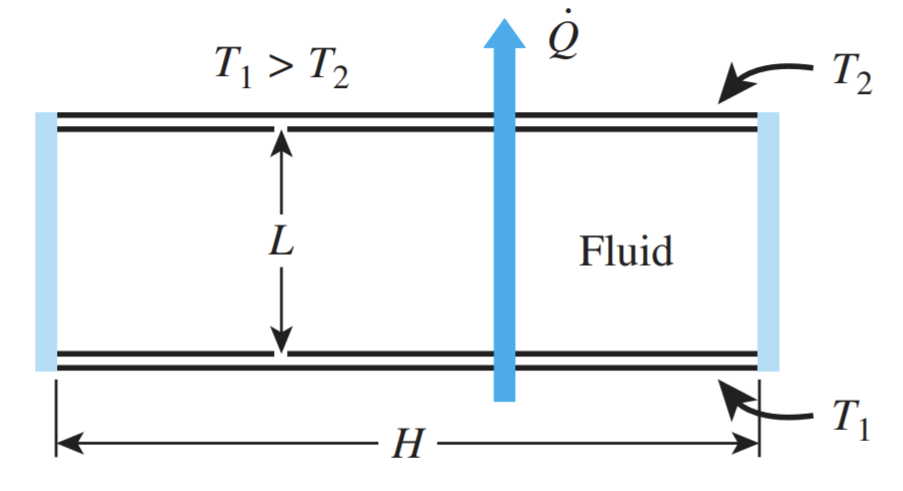
\includegraphics[width=8cm]{rbc_cengel.PNG}

        (Cengel 2015)
    \end{center}
\end{frame}

\begin{frame}[fragile]
    \frametitle{Why are we Still Studying Convection? \textbf{Applications}}
    \vfill
    % % \tikzart[t=m]{}% draw coordinate system
    % \tikzart[t=p,x=-6.3,y=-1.5,w=4]{earth-science-volcanoes-339345-1280x1024}{\fullcite{test}}% position picture
    % \tikzart[t=p,x=0,y=-1.5,w=4.2]{falk}% position picture
    % \tikzart[t=p,x=5,y=-1.5,w=4]{moto_fins}% position picture
    \begin{columns}
        \begin{column}{.30\textwidth}
            \centering
            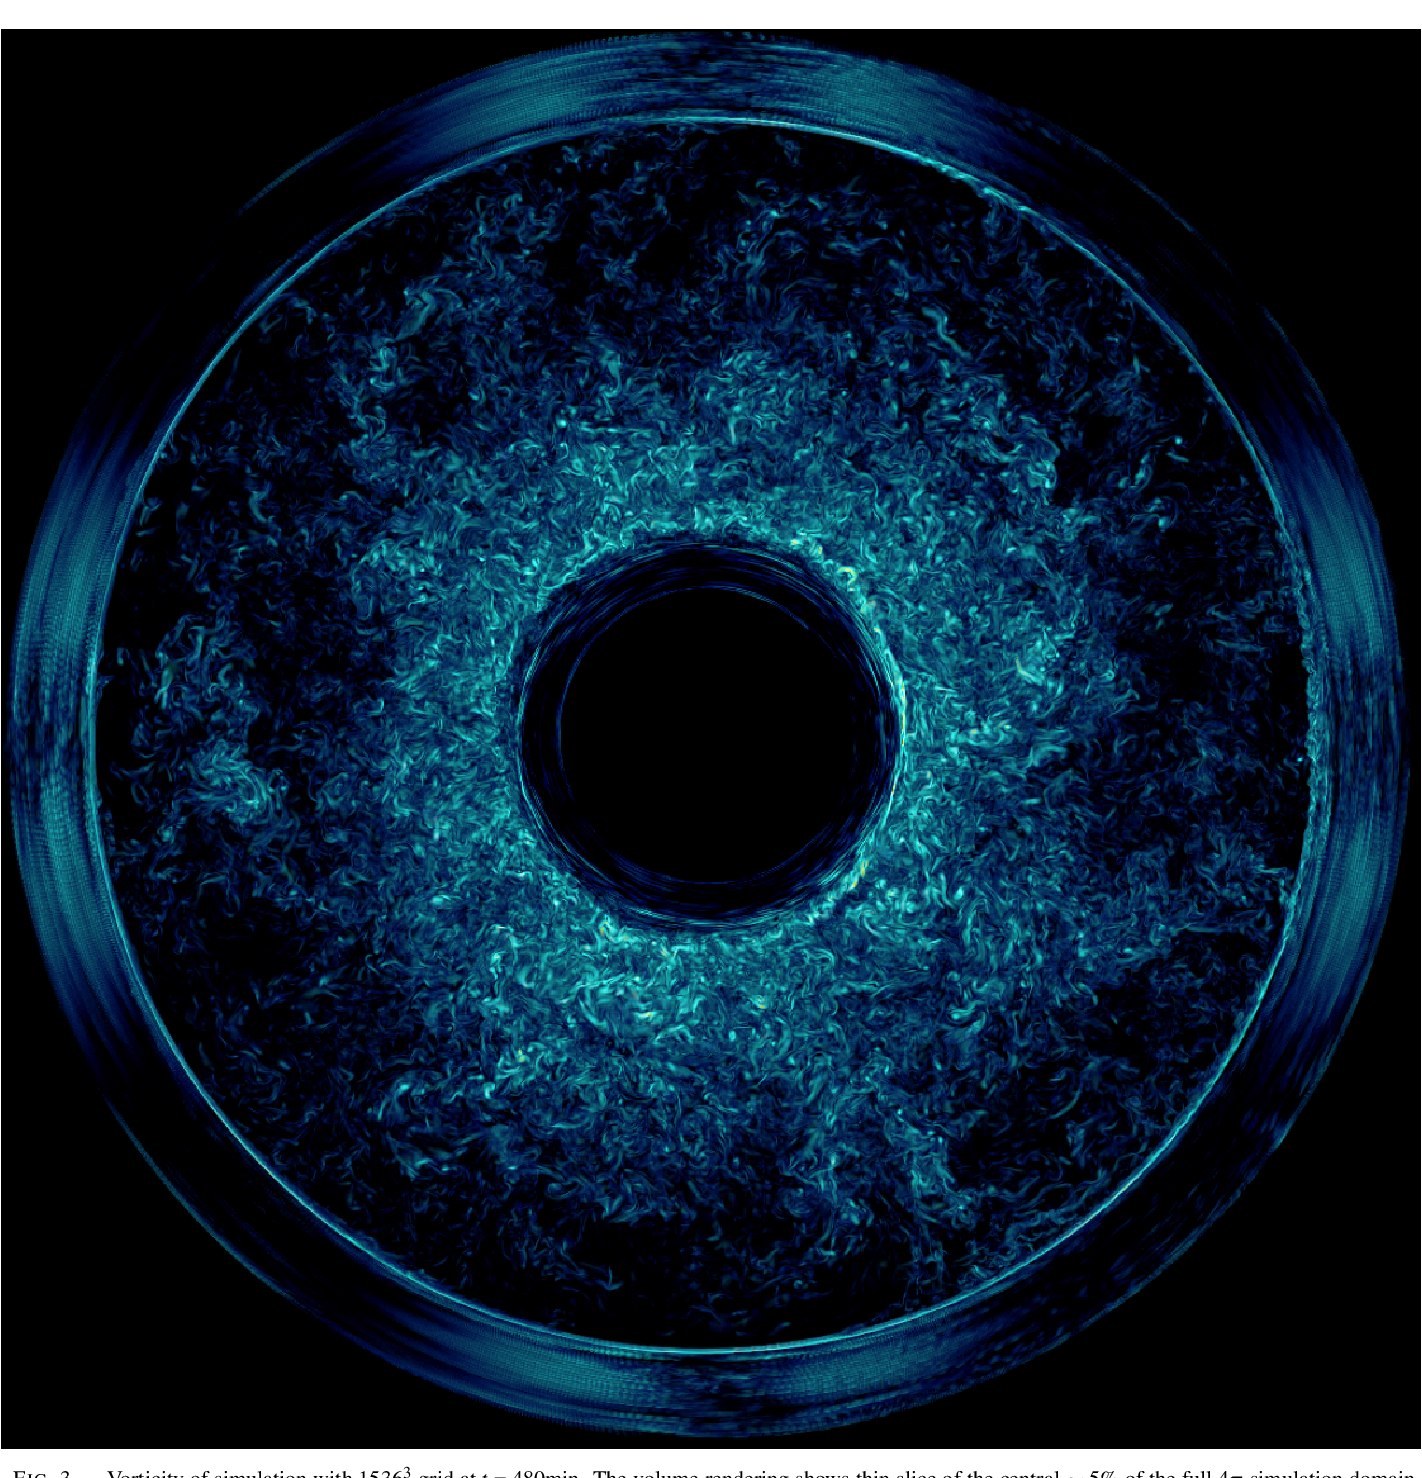
\includegraphics[height=0.8\textwidth]{falk.png}

            {Astrophysics}
        \end{column}

        \begin{column}{.3\textwidth}
            \centering
            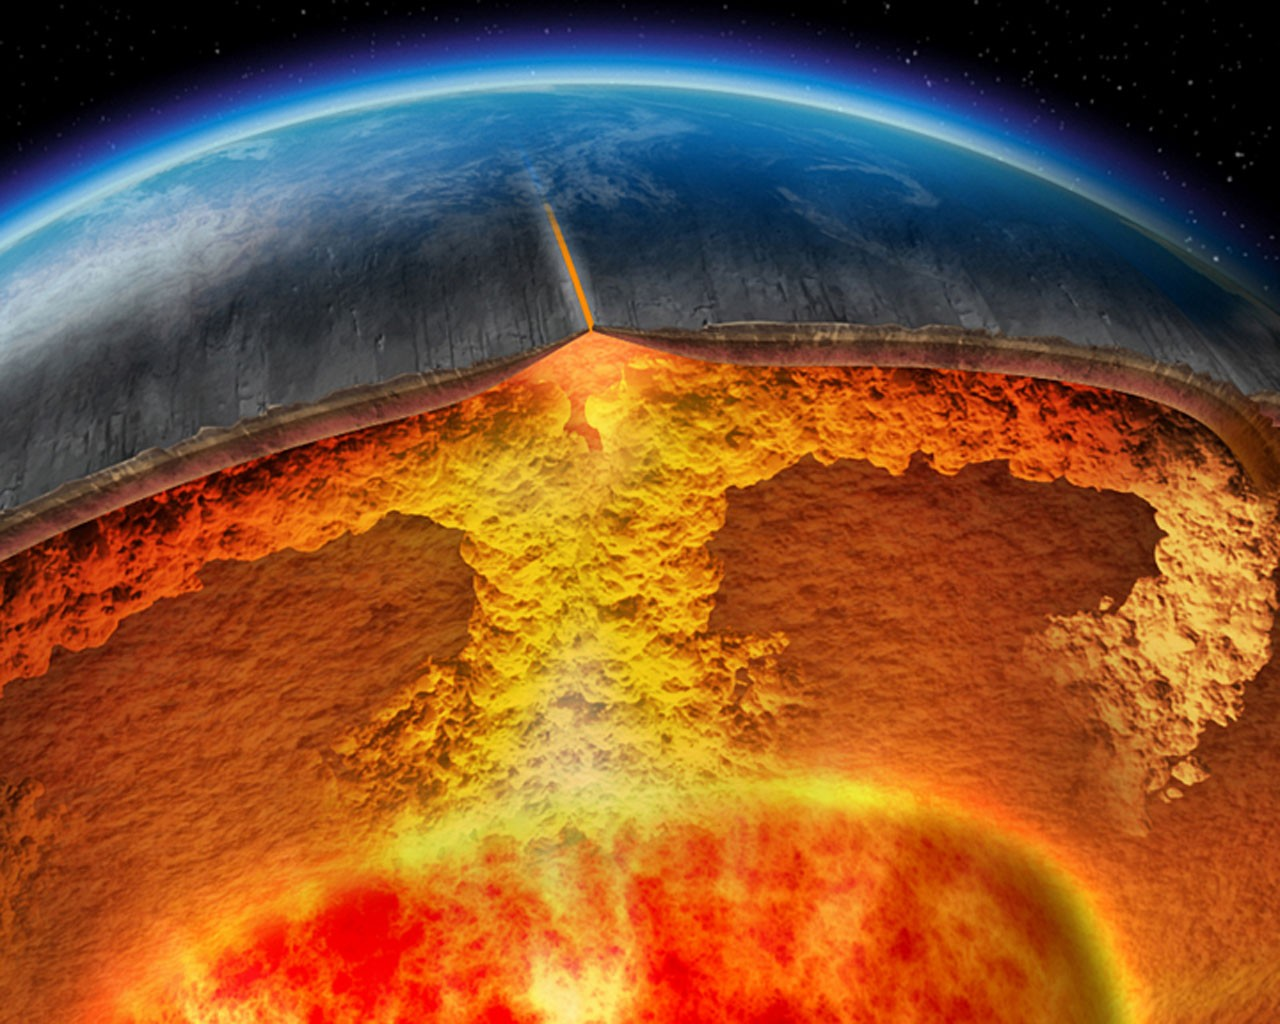
\includegraphics[height=0.8\textwidth]{earth-science-volcanoes-339345-1280x1024}

            {Geophysics}
        \end{column}

        \begin{column}{.30\textwidth}
            \centering
            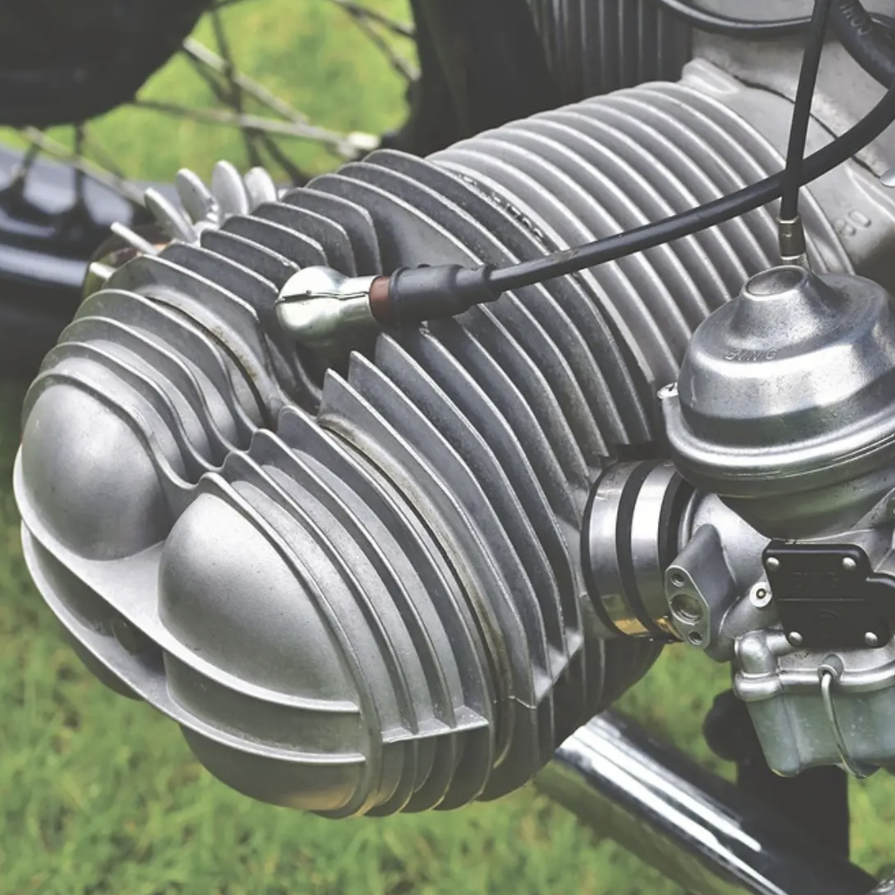
\includegraphics[height=0.8\textwidth]{moto_fins.png}

            {Engineering}
        \end{column}
    \end{columns}
\end{frame}

\begin{frame}[fragile]
    \frametitle{Why are we Still Studying Convection? \textbf{It's Elusive}}
    \vfill
    \begin{columns}
        \begin{column}{.30\textwidth}
            \centering
            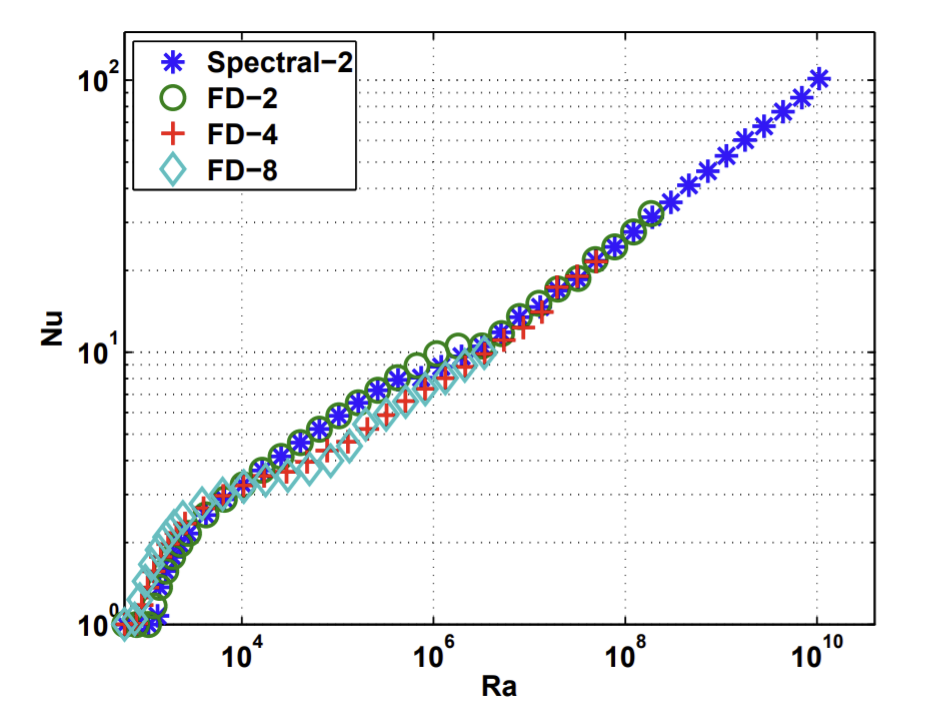
\includegraphics[height=0.85\textwidth]{johnson.png}

            {(Johnson and Doering 2009)}
        \end{column}

        \begin{column}{.60\textwidth}
            \centering
            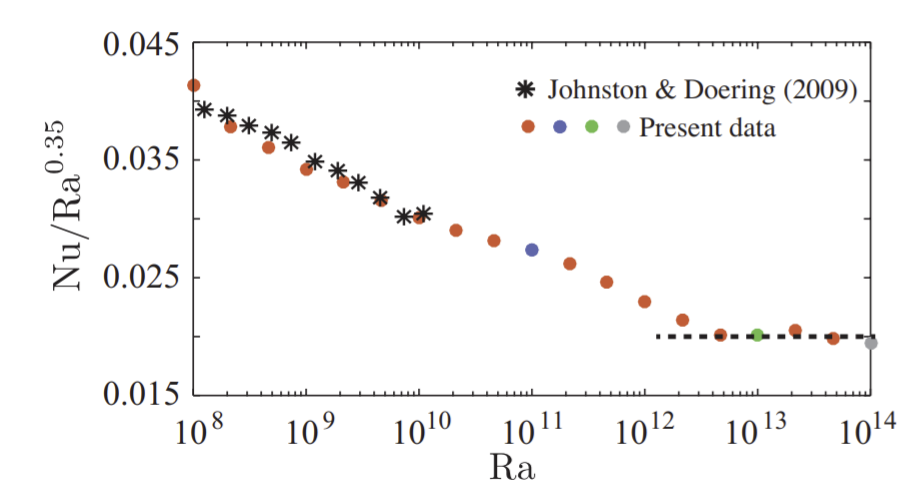
\includegraphics[height=0.5\textwidth]{zho.png}

            {(Zhu et al 2019)}
        \end{column}
    \end{columns}
\end{frame}

%---------------------------------------------------------------------------%

%---------------------------------------------------------------------------%
%
%---------------------------------------------------------------------------%
%->> Method
%---------------------------------------------------------------------------%
%---------------------------------------------------------------------------%
\lecture{Research Presentation}{lec_present_method}
%---------------------------------------------------------------------------%
\section{\enorcn{Methods}{研究方法}}
%---------------------------------------------------------------------------%
\begin{frame}[fragile]
    \frametitle{Rayleigh's Linear Stability Analysis}
    \begin{itemize}
        \item Assume variables can be decomposed like 
        \begin{align}
            \vec{u}(x, z, t) &= \vec{u'}(x, z, t) \label{EQ:reynolds_dc_u} = u'(x, z, t)\hat{x} + w'(x, z, t)\hat{z} \\
            T(x, z, t) &= \overline{T}(z, t) + T'(x, z, t) \label{EQ:reynolds_dc_T}\\
            p(x, z, t) &= \overline{p}(z, t) +  p'(x, z, t). \label{EQ:reynolds_dc_p}
        \end{align}
        \item The linear Eigenvalue Problem (EVP) is given by
        \begin{align}
            \nabla \cdot \vec{u'} &= 0 \label{EQ:linear1}\\
            \frac{\partial\vec{u'}}{\partial t} &= - \nabla p' + T'\hat{z} + \mathcal{R} \nabla^2 \vec{u'} \label{EQ:linear2}\\
            \frac{\partial T'}{\partial t} + \frac{\partial \overline{T}}{\partial z} w' &= \mathcal{P} \nabla^2 T' \label{EQ:linear3}
        \end{align}
    \end{itemize}
    
\end{frame}

\begin{frame}[fragile]
    \frametitle{Solutions to the Linear Problem}
        Solutions are given by
        \begin{align}
            w'(x, z, t) &= A\, \Re\left[W(z) \, e^{i(k_xx-st)}\right] \label{EQ:normal_modes1}\\ 
            u'(x, z, t) &= A\, \Re\left[U(z) \, e^{i(k_xx-st)}\right] \label{EQ:normal_modes2}\\ 
            T'(x, z, t) &= A\, \Re\left[\theta(z) \, e^{i(k_xx-st)}\right] \label{EQ:normal_modes3}\\ 
            p'(x, z, t) &= A\, \Re\left[P(z) \, e^{i(k_xx-st)}\right] \label{EQ:normal_modes4}
        \end{align}
        where $A$ is the (undetermined) mode amplitude, $s = \omega + i\sigma$ is the eigenvalue, \newline
        
        and the allowed wavenumbers $k_x \in \left\{\frac{n\pi}{2} \, \big| \, n \in \mathbb{N}\right\}$.
    
\end{frame}

\begin{frame}[fragile]
    \frametitle{The Quasilinear Model}
    \begin{itemize}
        \item The 1D quasilinear initial value problem (IVP)
        \begin{equation}
            \frac{\partial \overline{T}}{\partial t} + \frac{\partial}{\partial z} \langle w'T' \rangle_x = \mathcal{P} \frac{\partial^2 \overline{T}}{\partial z^2} \label{EQ:T0_IVP}
        \end{equation}
        \item Evolution due to \textbf{Advection}: $\frac{\partial}{\partial z} \langle w'T' \rangle_x $
        and \textbf{Diffusion}: $\mathcal{P} \frac{\partial^2 \overline{T}}{\partial z^2}$\newline

        \item Derived by manipulating the nonlinear and linear equations\newline
        
        \item Can be solved in conjunction with the EVP provided the amplitude $A$ is known\newline
        
        \hspace{0.5cm} $\mathbf{\longrightarrow}$ \textbf{Marginal Stability}

    \end{itemize}
    
    
\end{frame}

\begin{frame}[fragile]
    \frametitle{Marginal Stability Constraint}
    \begin{itemize}
        \item We assume the perturbations evolve on a shorter timescale than the background state\newline
        
        \item We impose \textbf{Marginal Stability} at each timestep
        \begin{equation}
            \max_{k_x} \{ \sigma \} = 0.
        \end{equation}

        \item The growth rate $\sigma$ is obtained by solving the EVP for some $\overline{T}(z,t)$\newline
        
        \item Does not allow us to solve for $A$ directly $\longrightarrow$ discrete root-finding methods
    \end{itemize}
    
\end{frame}

\begin{frame}[fragile]
    \frametitle{Solving for the Perturbation Amplitude $A$}
    \begin{enumerate}
        \item Given some guess for the amplitude $A$ and a fixed timestep $\Delta t$\newline
        
        \item We evolve the initial (marginally stable) temperature profile $\overline{T}(z,t) \; \xrightarrow{\text{IVP}} \; \overline{T}(z,t+\Delta t)$\newline
        
        \item Solve the EVP using $\overline{T}(z,t+\Delta t)$\newline
        
        \item This renders $\sigma(A)$\newline
        
        \item Use Newton's method with finite differences to solve $\sigma(A) = 0$
    \end{enumerate}
    
\end{frame}

\begin{frame}[fragile]
    \frametitle{The Amplitude Guess}
    \begin{itemize}
        \item Consider advection and diffusion separately on $t\;\to\; t+\Delta t$\newline
        
        \item Solve $\frac{\partial\overline{T}}{\partial t} + 2\frac{\partial}{\partial z} \Re\left[ W \theta^* \right] = 0$, yielding $\overline{T}_{adv} \; \xrightarrow{\text{EVP}} \; \sigma_{\rm{adv}}$\newline
        
        \item Solve $\frac{\partial\overline{T}}{\partial t} = \mathcal{P}\frac{\partial^2 \overline{T}}{\partial z^2}$, yielding $\overline{T}_{adv} \; \xrightarrow{\text{EVP}} \; \sigma_{\rm{diff}}$\newline
        
        \item For small timesteps, we assume diffusion and advection act independently, i.e.
        \begin{equation}
            0 = \Delta \sigma \approx A^2\sigma_{\rm{adv}} + \sigma_{\rm{diff}} \quad \longrightarrow \quad A^2 \approx -\frac{\sigma_{\rm{diff}}}{\sigma_{\rm{adv}}}
        \end{equation}
    
    \end{itemize}
    
\end{frame}
%---------------------------------------------------------------------------%

\begin{frame}[fragile]
    \frametitle{Multiple Marginally Stable Modes}
    \begin{itemize}
        \item Generalize
        \begin{equation}
            \langle w' T' \rangle_x = \sum_{n = 1}^{N} 2 A_n^2  \Re\left[ W_n \theta_n^* \right] 
        \end{equation}
        to accommodate $N$ simultaneously marginally stable modes\newline
        
        \item $N$ amplitudes ($\vec{A}\in\mathbb{R}^N$) to maintain marginal stability in $N$ modes
        \begin{equation}
            \vec{\sigma}(\vec{A}) = \vec{0}
        \end{equation} 
        \item Modes with negative amplitudes are not included
    \end{itemize}
    
\end{frame}
%---------------------------------------------------------------------------%

\begin{frame}[fragile]
    \frametitle{Solving for the Amplitude Vector $\vec{A}$}
    \begin{enumerate}
        \item Given some guess for the amplitude vector $\vec{A}$ and a fixed timestep $\Delta t$\newline
        
        \item We construct a Jacobian matrix with finite differences
        \begin{equation}
            J = \begin{bmatrix}
                \nabla \sigma_1 (A_1, A_2, ..., A_N) \\
                \nabla \sigma_2 (A_1, A_2, ..., A_N) \\
                \vdots \\
                \nabla \sigma_N (A_1, A_2, ..., A_N) 
            \end{bmatrix}.
        \end{equation}\newline

        \item Use Newton's method to solve $\vec{\sigma}(\vec{A}) = \vec{0}$
    \end{enumerate}
    
\end{frame}

\begin{frame}[fragile]
    \frametitle{The Amplitude Guess for $N$ modes}
    \begin{itemize}
        \item The amplitude vector can be approximated by
        \begin{equation}
            \vec{A^2} \approx = -\Sigma_{\rm{adv}}^{-1} \vec{\sigma_{\rm{diff}}}.
            \label{EQ:AN_approx}
        \end{equation}
        \item The advective growth rate matrix $\Sigma_{\rm{adv}}$ measures the effect of the $j$th mode's advection on the $i$th mode's growth rate\newline

        \item The diffusive growth rate vector $\vec{\sigma_{\rm{diff}}}$ measures the effect of diffusion on the $i$th mode's growth rate
    \end{itemize}
    
\end{frame}
%---------------------------------------------------------------------------%
%---------------------------------------------------------------------------%
\begin{frame}[fragile]
    \frametitle{Marginally Stable Thermal Equilibria}
    \begin{itemize}
        \item Evolve until the \textbf{advection} cancels \textbf{diffusion}
        \begin{equation}
            \frac{\partial}{\partial z} \langle w'T' \rangle_x = \mathcal{P} \frac{\partial^2 \overline{T}}{\partial z^2} \quad \longrightarrow \quad \frac{\partial \overline{T}}{\partial t} = 0
        \end{equation}

        \item Such states are referred to as Marginally Stable Thermal Equilibria (MSTE)\newline
        
        \item We compute symmetric MSTE for $10^6 \leq \rm{Ra}\leq 10^9$

    \end{itemize}
\end{frame}%
%---------------------------------------------------------------------------%
%->> Result
%---------------------------------------------------------------------------%
%---------------------------------------------------------------------------%
\lecture{Research Presentation}{lec_present_result}
%---------------------------------------------------------------------------%
\section{\enorcn{Results}{结果}}
%---------------------------------------------------------------------------%
\begin{frame}[fragile]
    \frametitle{\enorcn{Position animation + Make Table}{放置视频 + 制表}}
    \begin{center}
        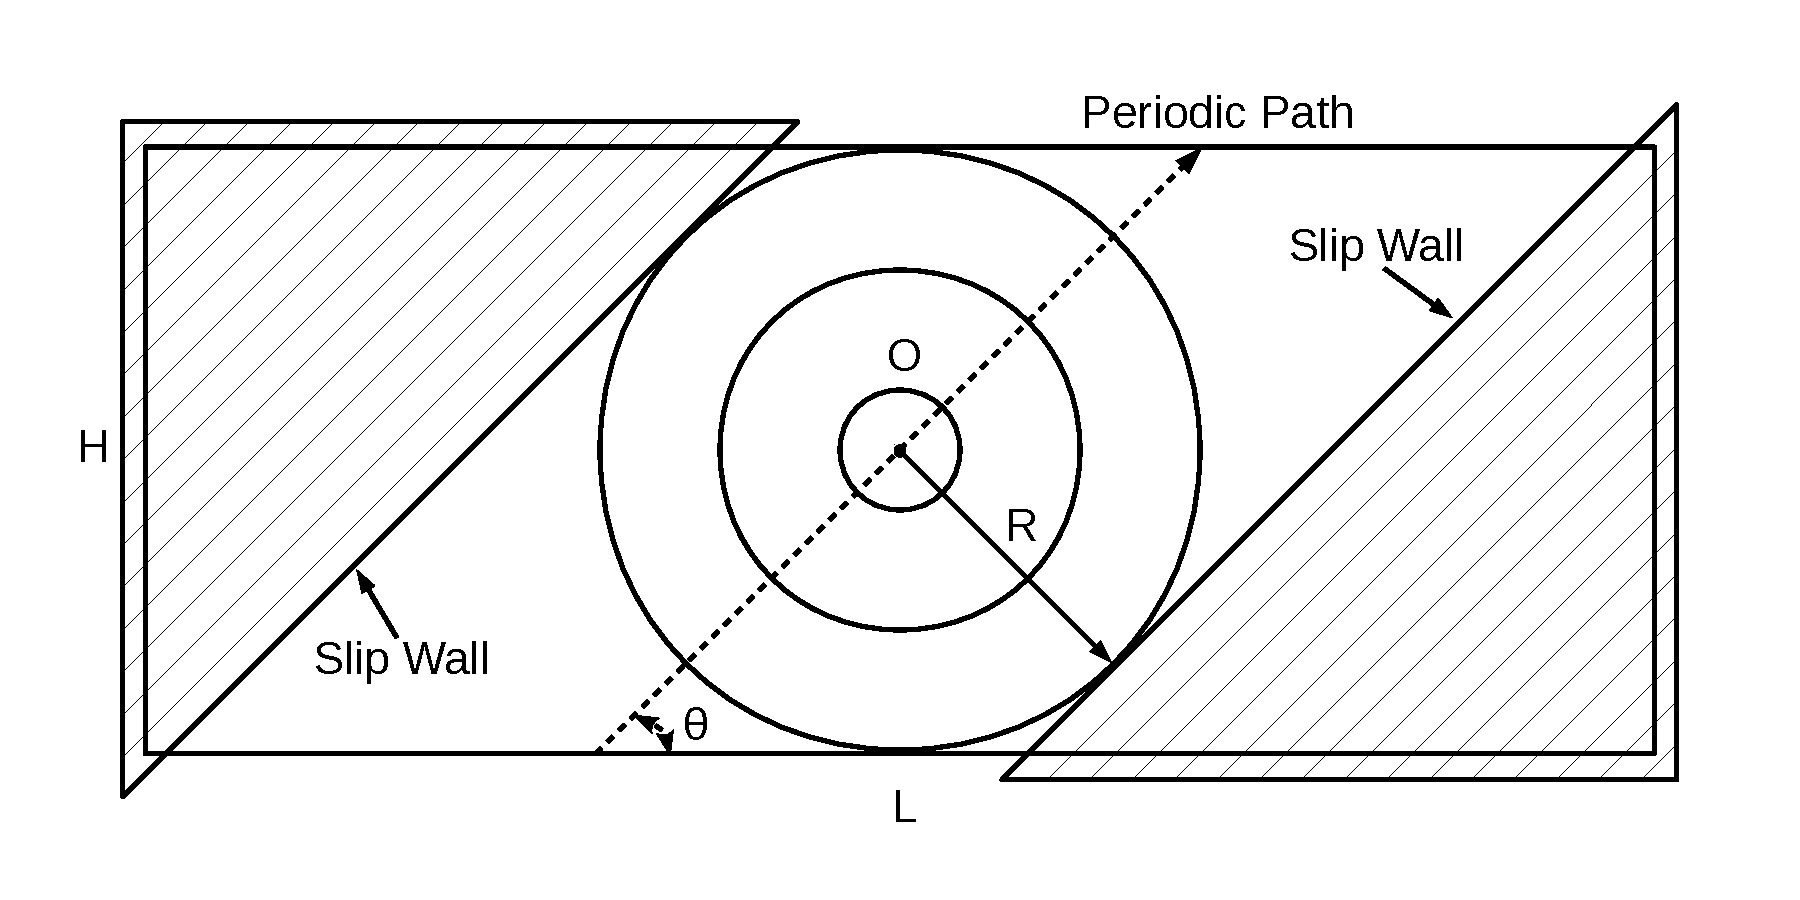
\includegraphics[trim=00mm 10mm 00mm 10mm,clip,width=0.4\textwidth]{vortex_preserve_demo}
    \end{center}

    \begin{center}
        \footnotesize
        \setlength{\tabcolsep}{3pt}
        %\renewcommand{\arraystretch}{1.5}
        \begin{tabular}{lc>{\columncolor[gray]{0.8}}cc>{\columncolor[gray]{0.8}}cc>{\columncolor[gray]{0.8}}c}
            \toprule
            %\multicolumn{2}{c}{Item} \\
            %\cline{1-2}
            $m_x \times m_y$ & $L_1$ error & $L_1$ order & $L_{2}$ error & $L_{2}$ order & $L_{\infty}$ error & $L_{\infty}$ order\\
            \midrule
            $40\times20$ & $3.536\mathrm{e}{-2}$ & $-$ & $6.097\mathrm{e}{-2}$ & $-$ & $4.105\mathrm{e}{-1}$ & $-$\\
            $80\times40$ & $9.113\mathrm{e}{-3}$ & $1.956$ & $2.497\mathrm{e}{-2}$ & $1.288$ & $1.997\mathrm{e}{-1}$ & $1.039$\\
            $160\times80$ & $2.034\mathrm{e}{-3}$ & $2.163$ & $6.548\mathrm{e}{-3}$ & $1.931$ & $5.236\mathrm{e}{-2}$ & $1.931$\\
            $320\times160$ & $5.114\mathrm{e}{-4}$ & $1.992$ & $1.640\mathrm{e}{-3}$ & $1.997$ & $1.278\mathrm{e}{-2}$ & $2.035$\\
            $640\times320$ & $1.287\mathrm{e}{-4}$ & $1.990$ & $4.097\mathrm{e}{-4}$ & $2.001$ & $3.119\mathrm{e}{-3}$ & $2.034$\\
            $1280\times640$ & $3.233\mathrm{e}{-5}$ & $1.993$ & $1.024\mathrm{e}{-4}$ & $2.000$ & $7.818\mathrm{e}{-4}$ & $1.996$\\
            \bottomrule
        \end{tabular}
    \end{center}
    \tikzart[t=v,x=9.5,y=-4.5,w=0.5]{Video/vortex_preserve_geo.mp4}[{\tiny$\color{gray}{\blacktriangleright}$}]% insert video

    \tikzart[t=t,x=6.5,y=2.5,w=4][draw=none,font=\tiny]{\enorcn{To play the video, the compiled PDF should be moved out from the "Tmp" directory}{播放视频时,编译生成的PDF需要从"Tmp"文件夹移出来}}% position text in the form of full citation
\end{frame}
%---------------------------------------------------------------------------%
%
%---------------------------------------------------------------------------%
%->> Conclusion
%---------------------------------------------------------------------------%
%---------------------------------------------------------------------------%
\lecture{Research Presentation}{lec_present_conclude}
%---------------------------------------------------------------------------%
\section{\enorcn{Conclusion}{结论}}
%---------------------------------------------------------------------------%
\begin{frame}[fragile]
    \frametitle{\enorcn{Ordinary text}{普通文本}}

    \begin{itemize}
        \item \textbf{A 3D, high-resolution, parallelized, gas-solid flow solver}
            \begin{itemize}
                    \footnotesize
                \item Establishes a numerical framework for the direct simulation of gas-solid flows.
                \item Solves coupled and interface-resolved fluid-fluid, fluid-solid, and solid-solid interactions.
                \item Addresses shocked flow conditions, irregular and moving geometries, and multibody contact and collisions.
            \end{itemize}
        \item\textbf{Advancement in understanding particle clustering and jetting}
            \begin{itemize}
                    \footnotesize
                \item Demonstrates a valid statistical dissipative property in solving explosively dispersed granular materials with respect to Gurney velocity.
                \item Extends the time range of the velocity scaling law with regard to Gurney energy in the Gurney theory from the steady-state termination phase to the unsteady evolution phase.
                \item Proposes an explanation for particle clustering and jetting instabilities to increase the understanding of experimental observations.
            \end{itemize}
    \end{itemize}
\end{frame}
%%---------------------------------------------------------------------------%
%
%---------------------------------------------------------------------------%
%
%-
%-> Backmatter
%-
%---------------------------------------------------------------------------%
%->> Backmatter
%---------------------------------------------------------------------------%
%->> Question
%---------------------------------------------------------------------------%
\lecture{Research Presentation}{lec_present_question}
%---------------------------------------------------------------------------%
{%
\begin{frame}[plain]
    \begin{center}
        {\large\bfseries {\enorcn{Thank you for your attention!}{感谢聆听!\par\medskip 敬请批评指正}}}
    \end{center}
    \tikzart[t=p,x=0,y=-4,w=4]{logo_uw}
    \addtocounter{framenumber}{-1}% modify the counter to exclude a frame from total count
\end{frame}
}
%---------------------------------------------------------------------------%
%->> Appendix
%---------------------------------------------------------------------------%
\lecture{Research Presentation}{lec_present_appendix}
%---------------------------------------------------------------------------%
\appendix% begin appendix
%\newcounter{finalframe}% define a new counter
%\setcounter{finalframe}{\value{framenumber}}% save regular slides counter
%---------------------------------------------------------------------------%
\section{\appendixname}% the end page.
\frame{\tableofcontents}% outline for appendix
%---------------------------------------------------------------------------%
\subsection{\enorcn{Classic Beamer Style}{常规Beamer风格}}
%---------------------------------------------------------------------------%
\begin{frame}[fragile]
    \frametitle{Sod's problem \parencite{sod1978survey}}

    \begin{columns}
        \begin{column}{.40\textwidth}
            \centering
            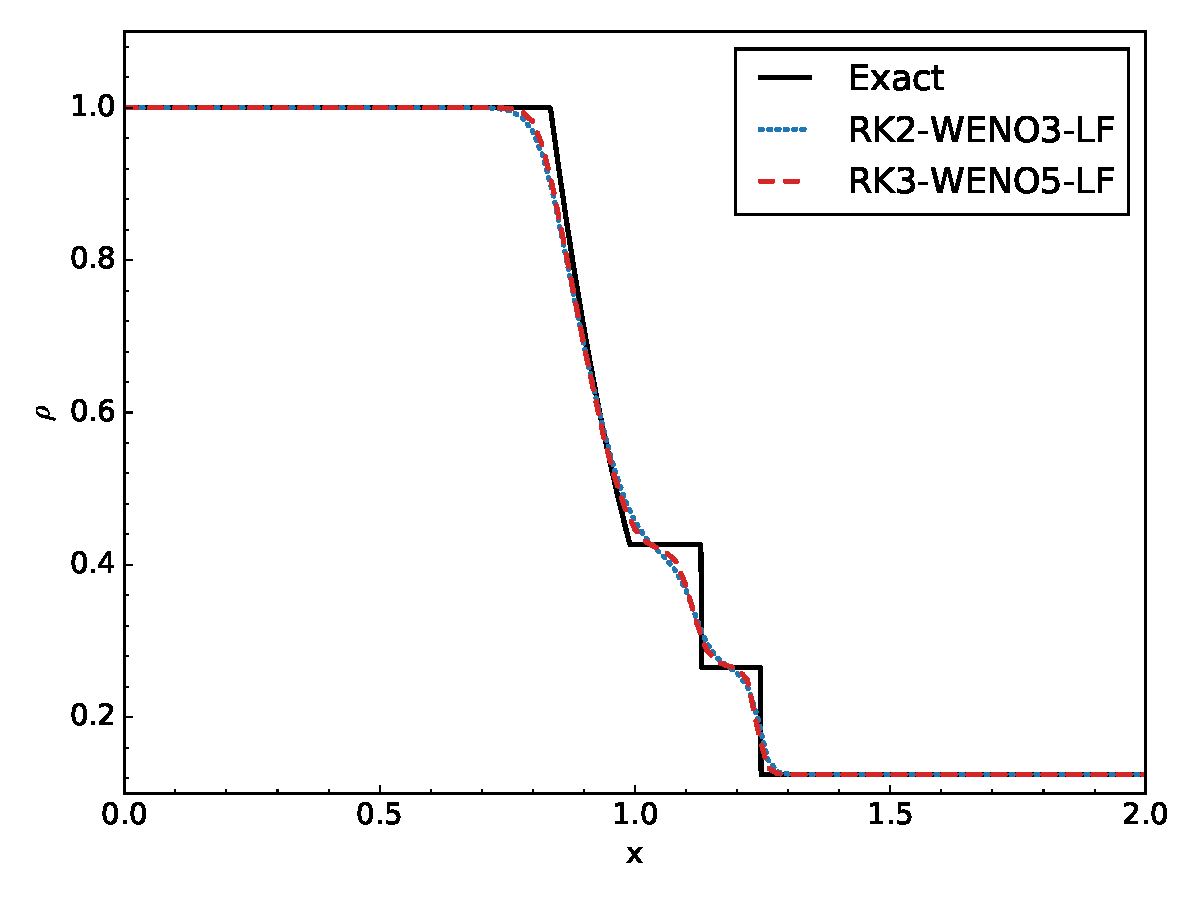
\includegraphics[width=\textwidth]{riemann_1d_sod_rho_x_n100}

            {$n=100$}
        \end{column}

        \begin{column}{.40\textwidth}
            \centering
            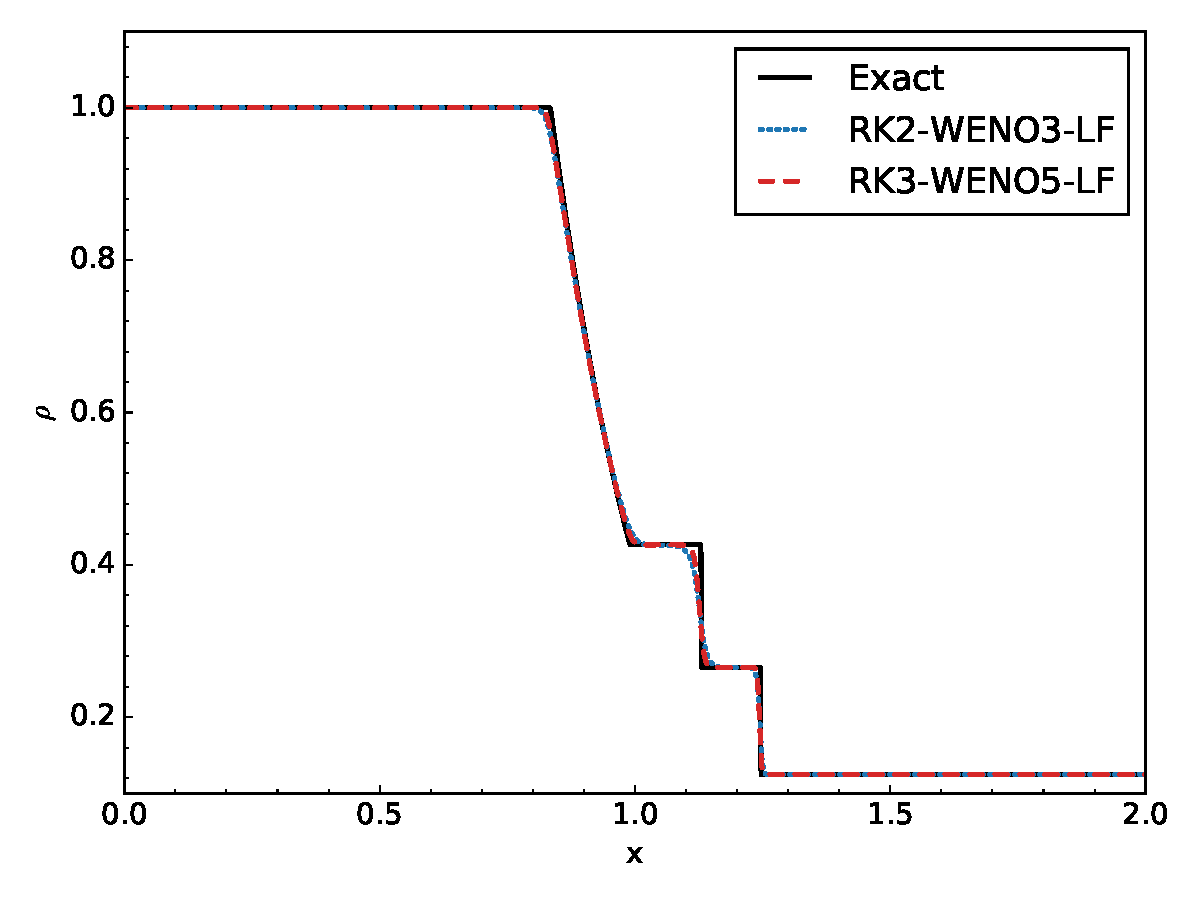
\includegraphics[width=\textwidth]{riemann_1d_sod_rho_x_n500}

            {$n=500$}
        \end{column}
    \end{columns}

    \bigskip\vfill

    \[
        \begin{gathered}
            \begin{aligned}
                \rho &= 1; & u &= 0; & p &= 1 & \ \text{if}\ & 0 \le x < 1 \\
                \rho &= 0.125; & u &= 0; & p &= 0.1 & \ \text{if}\ & 1 < x \le 2
            \end{aligned}
        \end{gathered}
    \]
\end{frame}
%---------------------------------------------------------------------------%
\lecture{Research Presentation}{lec_present_ref}
%---------------------------------------------------------------------------%
\subsection{\enorcn{References}{参考文献}}
%---------------------------------------------------------------------------%
\begin{frame}[allowframebreaks]
    \frametitle{References}
    \printbibliography[heading=none]%
\end{frame}
%---------------------------------------------------------------------------%
%\setcounter{framenumber}{\value{finalframe}}% rectify the slides counter
%---------------------------------------------------------------------------%
%
\end{document}
%---------------------------------------------------------------------------%
